\documentclass{standalone}
\usepackage{tikz}
\usepackage{ctex,siunitx}
\setCJKmainfont{Noto Serif CJK SC}
\usepackage{tkz-euclide}
\usepackage{amsmath}
\usetikzlibrary{patterns, calc}
\usetikzlibrary {decorations.pathmorphing, decorations.pathreplacing, decorations.shapes,}
\begin{document}
\small
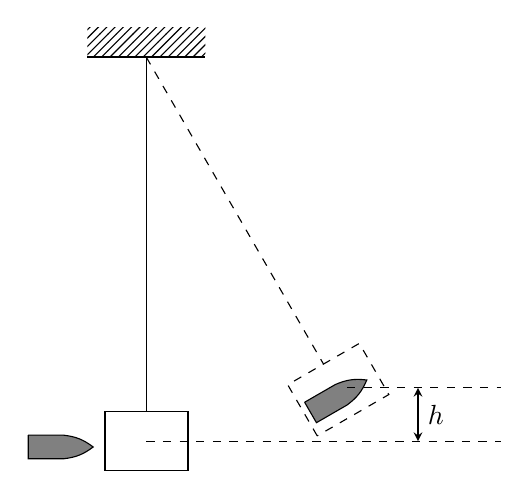
\begin{tikzpicture}[>=stealth,scale=1.5]
  \fill [pattern=north east lines](-.5,0) rectangle (.5,0.25);
  \draw [thick](-.5,0)--(.5,0);
  \draw [rotate=30, dashed] (-.35, -3.5) rectangle (.35, -3);
  \draw [semithick](-.35, -3.5) rectangle (.35, -3);
  \draw (0,0)--(-90:3);\draw[dashed] (0,0)--(-60:3);
  \draw[fill=gray] (-2+1, 5.3-8.5) --(-1.7+1, 5.3-8.5) to [bend left=15] (-1.45+1, 5.2-8.5) to [bend left=15] (-1.7+1,5.1-8.5)--(-2+1,5.1-8.5)--(-2+1,5.3-8.5); 
  \draw[rotate=30, fill=gray] (-2+1.7, 5.3-8.5) --(-1.7+1.7, 5.3-8.5) to [bend left=15] (-1.45+1.7, 5.2-8.5) to [bend left=15] (-1.7+1.7,5.1-8.5)--(-2+1.7,5.1-8.5)--(-2+1.7,5.3-8.5); 
  \draw [dashed](0,-3.25)--(3,-3.25);
  \draw [dashed](1.7,-2.8)--(3,-2.8);
  \draw[<->](2.3,-3.25)--node[right]{$h$}(2.3,-2.8);
\end{tikzpicture}
\end{document}